% !TEX root = diss.tex

 \chapter{Introduction}

Radicals are chemical species which tend to be highly reactive due to the
presence of one or more unpaired electrons. Living systems depend on radical
processes as part of normal metabolism but biological molecules, such as
proteins, are susceptible to radical induced damage. Radical induced oxidation
of biomaterials has been implicated in a number of degenerative disease states,
including cancer, Alzheimer's Disease, Parkinson's Disease, and multiple
sclerosis.\cite{Barnham2004,Halliwell2007,Valko2007,Hwang2013,Halliwell2015}

In biological systems, radicals are derived from both endogenous sources, such
as transition metal-ion redox processes and other \emph{in vivo} processes, as
well as exogenous sources, for instance, solar radiation and air pollutants.
Oxygen centred radicals, known as reactive oxygen species (ROSs) in biology, are
particularly important due to the nature of the aerobic respiration. The
radicals of primary concern are the highly reactive hydroxyl radical
(\ch{HO^.}), alkoxyl radicals (\ch{RO^.}), superoxide (\ch{HOO^.}/\ch{O2^{.-}}),
and peroxyl radicals (\ch{ROO^.}).\cite{Halliwell2015} Damage occurs when an ROS
initiates a radical chain reaction through hydrogen atom transfer (HAT),
electron transfer, or addition reactions, leading to rapid propagation. HAT is
the most relevant reaction and is the focus of my work.

Hydrogen atom transfer (HAT) reactions are a fundamental radical chemical
transformation which has been studied for over a
century.\cite{Kochi1973,Parsons2000} At the macroscopic level, HAT reactions
which involve oxygen centred radicals and non-radical organic substrates are
reasonably well characterised: the effects of bulk solvent are well
understood.\cite{Litwinienko2007} However, the roles of substrate-radical and
substrate-radical-medium interactions at the microscopic (molecular) level
continue to be relatively poorly understood. In my work, I shall make use of
quantum chemsitry in order to study HAT at the molecular level. In doing so, I
am able to develop a better understanding of the fundamental properties which
govern HAT reactions, and thus a develop insights into the many important
processes in which HAT takes place.

Recent work from our group, in collaboration with colleagues at University of
Rome Tor Vergata, has focused on the importance of substrate-radical
interactions. Specifically, it has been shown that the three-dimensional
structures of oxygen centred radicals, as well as the organic substrates,
impacts the nature of the interactions involved in HAT reaction pathways. In our
work, we utilise primarily the \bno and \cumo radicals, which serve as a
convenient proxy to biological oxygen centred radicals. Reaction involving \bno
and \cumo can be easily monitored using highly resolved laser flash photolysis
(LFP) techniques. A combination of theoretical and experimental techniques, have
been used to examine reactions involving \bno and \cumo with a variety of
organic substrates. A detailed discussion of these results shall be reserved for
following chapters, however, a great deal of insight has been gained into the
role of the structural of the radicals and substrates, and resulting
intermolecular interactions.

I have investigated several fundamental concepts associated with HAT reactions.
Firstly, in\iffalse~\ref{ch:arrheniuis}\fi Chapter 3 \jnote{update}, we shall
consider the well known, but phenomenological Arrhenius equation. Specifically,
I examine the relationship between the Arrhenius pre-factor and non-covalent
interactions. As of yet, there is no framework which relates the Arrhenius
pre-factor to the non-covalently bound pre-reaction complex. We hypothesise
there exists a direct correlation between the Arrhenius pre-factor and the
binding energy.

Secondly, we probe the applicability of the Bell-Evans-Polanyi (BEP) principle:
a linear free energy relationship which states that within a family of closely
related reactions, the reaction barrier heights are directly proportional to the
changes in enthalpy of reaction. We seek to determine how generally the BEP
principle can be applied by relating the highly-accurate theoretically
determined C-H bond strengths of species which undergo abstraction at these
positions to the experimentally determined HAT rate constants. HAT reaction rate
constants depend on many factors, however, by using measured rate constants from
specific conditions (LFP with \cumo at 298K), the difference in reactivity
depend mainly on the differences in chemical properties of the systems of
interest. Therefore, we hypothesise that there should exist two BEP
relationships for abstraction of C-H bonds: one in which the incipient radical
is delocalised into a $\pi$-system (benzylic/allylic) and the remaining
aliphatic C-H bonds.

Finally, recent experimental result show that non-redox active metal cations,
which are found ubiquitously in biological systems, have an inhibitory effect on
HAT reactions involving oxygen centred radicals and substrates which undergo
abstraction from sites adjacent to heteroatoms (e.g.\ amines, amides, and
ethers). Under various stoichiometric ratios, these metal cations have effects
ranging from full inhibition to partial deactivation of HAT
reactivity.\cite{Salamone2013,Salamone2015metals,Salamone2016} This effect has
been attributed partially to the effects of hyperconjugative overlap. Take for
example tetrahydrofuran (THF), shown in~\ref{fig:THF}. Normally, there exists
C-H bond weakening hyperconjugative overlap of electron density from one of the
oxygen lone-pairs and the adjacent C-H $\sigma^*$ anti-bonding orbitals. The
interaction of a metal cation with the oxygen lone-pairs removes electron
density from this interaction, thus increasing the C-H bond strength. As a
results, the reactivity of this bond is decreased, as observed from the
experimentally measured 3.2-fold decrease in the rate constant for HAT with
\cumo in acetonitrile from 6.65 \E{7} \Ms to 7.0 \E{7} \Ms in the presence of
1.0 M \ch{Mg(ClO4)2}.\cite{Salamone2013}

\begin{scheme}[htb]
  \centering
  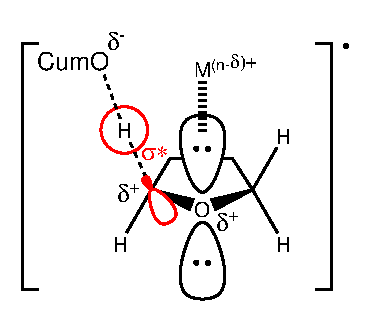
\includegraphics[width=0.65\textwidth]{figures/THF}
  \caption[Hyperconjugative overlap in tetrahydrofuran and the effect of non-redox active metal cations.]
  {Hyperconjugative overlap in tetrahydrofuran and the effect of non-redox active metal cations. The metal cation acts accepts electron density from the heteroatom lone pair, reducing overlap with the C-H $\sigma^*$ anti-bonding orbital and increasing the C-H bond strength.}
\label{fig:THF}
\end{scheme}

The nature of the interactions between non-redox active metal cations and
organic substrates is poorly understood. The primary goal of this thesis is to
understand the fundamental physico-chemical properties which lead to the
experimentally observed trends in reactivity. This problem is explored in
\iffalse\ref{ch:hat}\fi Chapter 5 \jnote{update}. The observed effects have led
us to hypothesise that the presence of non-redox active metal cations has a
chemoprotective effect against the radical induced oxidation of biomaterials
such as proteins.
